%!TEX root = main.tex

\title{Classification of distributed ternary labeling problems}
\author{Tanguy Rocher}
%!TEX root = main.tex
\documentclass[12pt]{report}

\usepackage{amsmath}
%\usepackage{gb4e}
\usepackage{natbib}
\usepackage{graphicx}
\usepackage{titlesec}
\usepackage{amssymb}
\usepackage{tcolorbox}
\usepackage{diagbox}
\usepackage{hyperref}
\usepackage[dvipsnames]{xcolor}
\hypersetup{
    colorlinks=true,
    linkcolor=blue,
    filecolor=blue,      
    urlcolor=blue,
}
\usepackage[utf8]{inputenc}
\usepackage[left=2cm, right=2cm, top=2cm]{geometry}
\usepackage[final]{pdfpages}
\usepackage{listings}%http://ctan.org/pkg/listings
\lstset{
  basicstyle=\ttfamily,
  mathescape
}

\usepackage{amsthm}
\theoremstyle{definition}
\newtheorem{exmp}{Example}[section]

\newcommand{\wdd}[0]{d}
\newcommand{\bdd}[0]{\delta}
 
\titleformat{\chapter}[display]{\normalfont\bfseries}{}{0pt}{\Huge}

\begin{document}
\maketitle

\tableofcontents
\newpage
\chapter{Ternary labeling problems}
%!TEX root = main.
In a previous work \cite{1} the class of binary labelling problem has been defined and classified according to the problem's complexity. This work aims to extend this classification to a larger class: the ternary labelling problems. The classification is not complete and focuses on ternary problems that have degrees $\wdd = 3$, $\bdd = 2$ even if a lot of the work done can also be applied to higher degrees. With this documentation, a classifier has been implemented (\href{https://github.com/trocher/tlpClassifier}{https://github.com/trocher/tlpClassifier}). Despite classifying problems, it also allows to look for a problem and its complexity. This work will show what the classifier is doing and prove its correctness, The latex source code of this document can be found on Github (\href{https://github.com/trocher/tlpDoc}{https://github.com/trocher/tlpDoc}).



\newpage
\chapter{The classifier}
%!TEX root = main.tex
\section{Generation of the problems}
\subsection{Non-reduced problem set}
We first generate all the possible white (resp. black) configurations by computing all the 3-tuple $(x_1,x_2, x_3)$ such that the 3 integer sum to $\wdd$ (resp. $\bdd$).
The powerset of this set will then be the set of all the possible \textit{white (resp. black) constraints}.
The cartesian product between the set of white constraints and the set of black constraints represent all possible problems. The following table represent the number of problems depending on $\wdd$ and $\bdd$
\begin{center}
\begin{tabular}{ | c | c | c | c |}
 \hline
 \diagbox{$\wdd$}{$\bdd$} & 2 & 3 & 4 \\ 
 \hline
 2 & 4096 & 65536 & 2097152\\
 \hline
 3 &  & 1048576 & 33554432\\
 \hline
 4 &  &  &  1073741824\\
\hline
\end{tabular}
\end{center}
\subsection{Representative problem set}
In order to reduce the data set and avoid to classify problems that are equivalents, for each equivalence set of problems, we can only keep the representative problems in the problem set. This lead to the following number of problems presented in the following table, still depending on $\wdd$ and $\bdd$
\begin{center}
\begin{tabular}{ | c | c | c | c |}
 \hline
 \diagbox{$\wdd$}{$\bdd$} & 2 & 3 & 4 \\ 
 \hline
 2 & 430 & 11456 & 353664\\
 \hline
 3 &  & 88792 & ?\\
 \hline
 4 &  &  &  ?\\
\hline
\end{tabular}
\end{center}

We can observe a set of problems 6 times smaller when $\wdd \neq \bdd$ (due to removing 5 of the 6 different permutations of the configurations tuples to only keep the characteristic problem) and 12 times smaller when $\wdd=\bdd$ due to the additional white/black symmetry

\subsection{The constraint reduction algorithm}\label{sec:CR}

\subsubsection{The algorithm}
We are going to introduce an algorithms that, when applied to each of the problems of the data-set, will reduce its size again considering that a problem with a "useless" configurations has an equivalent complexity of the same problem reduced to only its "useful" configurations.\\

The algorithm consist in removing all the white and black configurations of a problem that cannot be used by any node by the problem. It appear that it can be used to show the solvability of a problem as it will be showed later, however it is also useful to have a better understanding of a problem still unclassified.
\begin{itemize}
    \item The algorithm take as input a problem $\Pi = (\wdd,\bdd,W,B)$
    \item We start by looking at the set $S$ of labels that are in $A_{\Pi}$ but not in  $A_{\Pi,w} \cap A_{\Pi,b}$.
    \item For each labels $l$ present in $S$ we know that no node can use a configuration containing $l$ since one of its neighbors would have to have a corresponding configurations also containing $l$ which is impossible by construction of $S$.
    \item We hence know that all the white or black configurations containing any labels of $S$ will never be used, we can then safely remove them from the white and black constraint sets without modifying the problem.
    \item It is now possible to repeat this procedure on the new white and black constraints sets obtained until either one of them is empty or $S$ is empty
\end{itemize}
\begin{exmp} Constraint reduction algorithm on $\Pi = (3, 2, \{AAA, ABA\}, \{AA, CB, CC\})$

In the first iteration, we have $S = \{C\}$ since there is no configuration with $C$ in $W$ while there is one in $B$.
This lead us to remove both $CC$ and $CB$ from $B$ since no white node could properly label if one of its black neighbor would label their common edge with a $C$.
The new constraints set are :
$$W' = \{AAA, ABA\}, B' = \{AA\}$$
By running another iteration of the algorithm we get $S = \{B\}$ since $CB$ has been removed from $B$ in the previous iteration.
This hence lead to remove $ABA$ from $W$ since this time a black node could not properly label its edge if it is adjacent to a white node that label their common edge with a $B$.
The new constraints set are :
$$W' = \{AAA\}, B' = \{AA\}$$
This time, the algorithm return $S = \{\}$, it hence finish and return the following problem $\Pi' = (3, 2, \{AAA\}, \{AA\})$, which is equivalent to $\Pi$.
\end{exmp}

\begin{exmp} Constraint reduction algorithm on $\Pi = (3, 2, \{ABB, ABA, BBB\}, \{AA, CB, CC\})$

In the first iteration, we have $S = \{C\}$ since there is no configuration with $C$ in $W$ while there is one in $B$.
This lead us to remove both $CC$ and $CB$ from $B$ since no white node could properly label if one of its black neighbor would label their common edge with a $C$.
The new constraints set are :
$$W' = \{ABB, ABA, BBB\}, B' = \{AA\}$$
By running another iteration of the algorithm we get $S = \{B\}$ since $CB$ has been removed from $B$ in the previous iteration.
This hence lead to remove $ABB$, $ABA$ and $BBB$ from $W$ since this time a black node could not properly label its edge if it is adjacent to a white node that label their common edge with a $B$.
The new constraints set are :
$$W' = \{\}, B' = \{AA\}$$
$W'$ is empty, the algorithm hence finish and return the following problem $\Pi' = (3, 2,\{\}, \{AA\})$, equivalent to $\Pi$, this problem is obviously not solvable, the utility of the constraint reduction in proving the solvability of a problem will be showed later when classifing the unsolvable problems.
\end{exmp}
\subsubsection{Improvement on the size of the problem set}

Using the algorithm reduce the number of problems to classify since a lot of them are reduced to some same problems, this lead to the following number of problems presented in the table, again depending on $\wdd$ and $\bdd$:
\begin{center}
\begin{tabular}{ | c | c | c | c |}
 \hline
 \diagbox{$\wdd$}{$\bdd$} & 2 & 3 & 4 \\ 
 \hline
 2 & 248 & 7962 & \\
 \hline
 3 &  & 81694 & ?\\
 \hline
 4 &  &  &  ?\\
\hline
\end{tabular}
\end{center}


\section{Classification of a problem}
We are going to classify the problems into the 5 following categories : \textit{constant, iterated-logarithmic, logarithmic, global, unsolvable}. To classify a problem $\Pi$ in a category $c$, one should show that $\Pi$  have $c$ as lower bound on its complexity (in other world, it is not possible to solve $\Pi$ in $o(c)$ and that $\Pi$ has $c$ as upper bound on its complexity ($\Pi$ is solvable in $O(c)$). Since a lot of problems are relaxations or restriction of other problems, we are going to use this fact to "propagate" lower and upper bound in the following way.
\subsection{Giving a lower bound to a problem}
Suppose we have some lower-bound of the complexity $l$ of a problem $\Pi$. We should follow the following steps:
\begin{itemize}
    \item If the problem had a previously attributed lower-bound on the problem that was smaller than the new one, replace it by $l$ if it had a previously attributed upper-bound that is smaller than the new lower-bound, there must be an error.
    \item For all the problems that are a restriction of any problems of the set of equivalent problems of $\pi$, set its lower-bound to $l$
\end{itemize}
\subsection{Giving a upper bound to a problem}
Suppose we have some upper-bound of the complexity $u$ of a problem $\Pi$. We should follow the following steps:
\begin{itemize}
    \item If the problem had a previously attributed upper-bound on the problem that was bigger than the new one, replace it by $u$
    \item For all the problems that are a relaxation of any problems of the set of equivalent problems of $\pi$, set its upper-bound to $u$
\end{itemize}
Setting a complexity $c$ to a problem is then similar to applying both of theses process to the problem.


\section{The classification of binary labelling problems}\label{sec:BLP}
A complete complexity classification of the problems using 1 or 2 labels already exists \cite{1}. In the case of the problems that are using 3 labels theses result will be useful in two ways :
\begin{itemize}
    \item Since ternary labelling problems are always relaxation of some binary labelling problems, it provide some useful upper bounds for problems with 3 labels.
    \item As we will see, some 3-labelling problems can be reduced to 2-labelling problems since some of their labels are in fact redundant.
\end{itemize}
\subsection{Implementation of the binary labelling problems}
The entire results of the binary labelling problems has been implemented in the classifier, despite providing nice upper bounds for ternary labelling problems, it is also possible to query the complexity of a binary labelling problem with white and black degrees unbounded.
\subsubsection{Redundant labels}
The idea here is that in some problems with $|A_{\Pi}|=3$, we could create a new problem with the same complexity by removing every configuration that use a label $l_i$.\\
In order to do that, there must be a label $l_j\neq l_i$ such that for every configuration $c=(x_{l_1},x_{l_2},x_{l_3})$ using $l_i$, there must exists another configuration $c'=(x_{l_1'},x_{l_2'},x_{l_3'})$ such that : 
\begin{itemize}
    \item $l_i'=0$
    \item $l_j'= l_j+l_i$
    \item $l_k' = l_k$ where $ k = \Sigma \setminus \{l_i,l_j\}$ 
\end{itemize}
In other word, each time a node is using a configuration using $l_i$ it could safely switch to a similar configuration using $l_j$ instead of $l_i$. Hence it appear that if we remove all the configurations using $l_i$ the new binary labelling problem obtained will have the same complexity since $l_i$ was redundant.
The constructed problem cannot be easier than the original one since it is a restriction of it.
\begin{exmp}
Let $\Pi$ be the following problem with $\wdd = 3$ and $\bdd = 2$ :
\begin{itemize}
    \item $W = ABB, BBC, BCC, CCC, AAA, BBB, ACC, ABC$
    \item $B = AC, AB$
\end{itemize}
Can be described as :
Let's show that C is redundant in this problem and can be replaced by B:\\\\
In the black constraint, $AC$ is the only configuration using $C$, we can use $AB$ instead (the $C$ is replaced by $B$\\
In the white constraint :
\begin{itemize}
    \item $BB\textbf{C} \rightarrow BB\textbf{B}$
    \item $B\textbf{CC} \rightarrow B\textbf{BB}$
    \item $\textbf{CCC} \rightarrow \textbf{BBB}$
    \item $A\textbf{CC} \rightarrow A\textbf{BB}$
    \item $AB\textbf{C} \rightarrow AB\textbf{B}$
\end{itemize}
We can see that each new configuration obtained by replacing $C$ by $B$ is indeed in the black constraint.\\
We can now construct a binary labelling problem $\Pi'$ equivalent to $\Pi$ :\\
$\Pi'=(3,\bdd,W',B')$ with :
\begin{itemize}
    \item $W' = ABB, AAA, BBB$
    \item $B' = AB$
\end{itemize}
W' and B' being W and B minus all the configurations using $C$
\end{exmp}

\newpage
\chapter{Unsolvable problems}
%!TEX root = main.tex
\section{The constraint reduction}
The Constraint Reduction algorithm presented \hyperref[sec:CR]{\textbf{previously}} can show the solvability of a given problem, we will show it here.\\\\
Let's take a problem $\Pi = (\wdd,\bdd,W,B)$. After running the constraint reduction algorithm on $\Pi$, we obtain an equivalent problem $\Pi' = (\wdd,\bdd,W',B')$ we can have two different outputs :
\begin{itemize}
    \item $|W'| = 0$ or $|B'| = 0$ :
    
    In this case, it seems pretty obvious that $\Pi' = (\wdd,\bdd,W',B')$ cannot be solved since that we cannot assign any configuration to either the white nodes or the black nodes, because $\Pi'$ is equivalent to $\Pi$. It appears that $\Pi$ is unsolvable as well.
    \item  $|W'| > 0$ and $|B'| > 0$:
    
    In this case, we are going to prove that $\Pi$ must be solvable by showing an algorithm that solve it:
    \begin{itemize}
        \item We elect a white leader in the graph using $GATHER$
        \item The leader chooses any configuration in $W'$ (this is possible since $|W'|>0)$
        \item Each time a white (resp. black) node $u$ in the graph has a complete labelling of its adjacent edges, it sends, to each of its neighbors $v_i$, $i\in\wdd$ (resp. $i\in\bdd$) the label $l$ of their common edge $(u,v_i)$. $u$ does not do anything else afterwards.
        \item Each time a white (resp. black) node $v$ receives such a label $l$, it finds a configuration $c$ in $W$ (resp. $B$) that contains $l$ and labels all its other incident edges with the other labels of $c$. Note that finding such a configuration is possible since by construction, if $W'$(resp. $B'$) contains a configuration with $l$, $B'$ (resp. $W'$) must contain a configuration with $l$
    \end{itemize}
\end{itemize}

At some point, the graph should be fully labelled even if it took $\mathcal{O}(n)$ time to do it. Remember that since the graph is a tree, a given un-visited node can only have 1 neighbor that has labelled their common edge at some point of time, there is hence no conflict in the labelling.

\section{Results}
The constraint reduction algorithm can be used with any white and black degree, however we are here focusing on $\wdd = 3, \bdd = 2$.
As explain above, the algorithm leads to a fully classification of the unsolvable problems, the other problems must have a complexity  $\mathcal{O}(n)$. In the case $\wdd = 3, \bdd = 2$, we found that 227 out of 7962 problems are unsolvable.

\newpage
\chapter{Global problems}
%!TEX root = main.tex
Now that all unsolvable problems have been classified, we know that every problem left must have a $\mathcal{O}(n)$ complexity. In this section, we are going to try to show that  $\Omega(n)$ hold on the complexity of some problems (which would lead the problem to be $\Theta(n)$).
\section[Proving Omega(n)]{Proving $\Omega(n)$}
The binary labelling problem classification described in section \ref{sec:BLP} is implemented and shows that $\Omega(n)$ hold for a lot of problems. Indeed, while some problems $\Pi$ having a global complexity are classified since $|A_\Pi|<3$, some other with $|A_\Pi| = 3$ are classified using the redundancy of their labels. In the case of $\wdd = 3, \bdd = 2$, this leads to the classification of 153 problems having a global complexity.


\newpage
\chapter{Constant problems}
%!TEX root = main.tex
\section{The round eliminator}
\subsection{Constant upper bound}
Before going any further, we will reduce the database set by removing from it a lot of constant problems.
By using round-elimination \cite{round-eliminator}, we are able to get constant upper bounds on a lot of problems. The round-eliminator can prove that a given problem must have a constant complexity, however, a problem for which the round-eliminator does not find a constant upper bound can also be constant.

Since the time and resources needed by the round eliminator are increasing with the \textit{iterations} and \textit{labels} parameters, we run the round eliminator on the set of unclassified problem by iteration while increasing the parameters each time.

With $\wdd = 3$, $\bdd = 2$, and by using the auto upper bound functionality of the tool, we manage to classify 6472 constant problems with the following distribution on their upper bound.
\begin{itemize}
    \item 0 rounds : 5414 problems
    \item 1 rounds : 761 problems
    \item 2 rounds : 65 problems
    \item 3 rounds : 138 problems
    \item 4 rounds : 16 problems
    \item 5 rounds : 37 problems
    \item 6 rounds : 15 problems
    \item 7 rounds : 15 problems
    \item 8 rounds : 8 problems
    \item 9 rounds : 3 problems
\end{itemize}

\subsection{Constant lower bound}
The round eliminator \cite{round-eliminator} also provides an automatic lower bound feature, we used it on the constant problems that are not 0 rounds solvable according to the upper bounds found earlier to get nice constant lower bounds and get the following distribution with the parameters $\wdd = 3$, $\bdd = 2$ :
\begin{itemize}
    \item 6 rounds : 2 problems
    \item 5 rounds : 17 problems
    \item 4 rounds : 57 problems
    \item 3 rounds : 156 problems
    \item 2 rounds : 65 problems
    \item 1 rounds : 761 problems
    \item 0 rounds : 5414 problems
\end{itemize}

Please note that since we ran the automatic upper and lower bound features with both the black and white node as active nodes, for each problem, we kept the smallest upper bound found. As for the lower bound, we kept the biggest one found such that it is smaller or equal than the upper bound of the problem.

\newpage
\chapter{Logarithmic problems}
%!TEX root = main.tex

\section{Known logarithmic problems}
\subsection{The 3-vertex coloring}
It is known that d-vertex coloring has a complexity $\Theta(log_dn)$ on d-regular trees \cite{DBLP:journals/corr/ChangKP16}, therefore we can classify the 3-vertex coloring problem on 3-regular trees: $$W = \{AB, AC, BC\}, B =\{AAA,BBB,CCC\}$$


\subsection{The 3-edge coloring}
First, we know that d-edge coloring has a complexity $\mathcal{O}(log_dn)$  on d-regular trees with $d\geq 3$ \cite{DBLP:journals/corr/abs-1708-04290}.
We also know that 3-edge coloring has a complexity $\Omega(log_n)$ on 3-regular trees \cite{balliu2019locality}, we can then classify the 3-edge coloring problem on 3-regular trees: $$W = \{AA, BB, CC\}, B=\{ABC\}$$


\section{Logarithmic upper bound using sinkless and sourceless orientation}
From \cite{1} we know that creating a sinkless and sourceless orientation (SSO) in a 3 regular has a $\Theta(log(n))$ complexity \cite{1}. Let use this result to show that some 3 labelling problems have a $\mathcal{O}(log(n))$ complexity. To do that, for each problem, we will show that given any graph with a SSO, there exist a constant algorithm that solve it.\\
The SSO ensure that, on any 3 regular graph, a given node $u$ with a degree 3 has either:
\begin{itemize}
    \item 2 outgoing edges and 1 incoming edge
    \item 1 outgoing edge and 2 incoming edges
\end{itemize}
The former will be denoted $X$ when the latter $Y$
\subsection[(W = (ABC, BCC), B = (AC,BC)]{$W = \{ABC, BCC\}$, $B = \{AC, BC\}$}
\begin{itemize}
    \item We label the nodes of type $X$ with $BCC$ such that the port corresponding to the incoming edge is labelled with $B$
    \item We label the nodes of type $Y$ with $ABC$ such that the port corresponding to the outgoing edge is labelled with $C$
\end{itemize}
The white constraint is respected since there are no other configuration used for any node with a degree 3.
We can see that any oriented edge $(u,v)$ start from a port of $u$ labelled with a $C$ and can either end on a port of $v$ labelled with $A$ or $B$, since the black constraint contains both $AC$ and $BC$ in both of theses cases the configuration is valid.
\subsection[(W = (AAB, BBC), B = (AB,BC)]{$W = \{AAB, BBC\}$, $B = \{AB, BC\}$}


\begin{itemize}
    \item We label the nodes of type $X$ with $BBC$ such that the port corresponding to the incoming edge is labelled with $C$
    \item We label the nodes of type $Y$ with $AAB$ such that the port corresponding to the outgoing edge is labelled with $B$
\end{itemize}
The white constraint is respected since there are no other configuration used for any node with a degree 3.
We can see that any oriented edge $(u,v)$ start from a port of $u$ labelled with a $B$ and can either end on a port of $v$ labelled with $A$ or $C$, since the black constraint contains both $BA$ and $BC$ in both of theses cases the configuration is valid.



\section{Logarithmic upper bound using even orientation}
Again, from \cite{1} we know that creating an even orientation (EO) in a 3 regular has a $\Theta(log(n))$ complexity \cite{1}. Let use this result to show that some 3 labelling problems have a $\mathcal{O}(log(n))$ complexity. To do that, for each problem, we will show that given any graph with a EO, there exist a constant algorithm that solve it.\\
The EO ensure that, on any 3 regular graph, a given node $u$ with a degree 3 has either:
\begin{itemize}
    \item 2 outgoing edges and 1 incoming edge
    \item 0 outgoing edge and 3 incoming edges
\end{itemize}
The former will be denoted $X$ when the latter $Y$
\subsection[(W = (ABC, CCC), B = (AC,BC)]{$W = \{ABC, CCC\}$, $B = \{AC, BC\}$}
\begin{itemize}
    \item We label the nodes of type $X$ with $ABC$ such that the port corresponding to the incoming edge is labelled with $C$
    \item We label the nodes of type $Y$ with $CCC$
\end{itemize}
The white constraint is respected since there are no other configuration used for any node with a degree 3.
We can see that any oriented edge $(u,v)$ start from a port of $u$ labelled with either $A$ or $B$ and end on a port of $v$ labelled with $C$, since the black constraint contains both $AC$ and $BC$ in both of theses cases the configuration is valid.

\subsection[(W = (X0X1X2, X3CC), B = (AC,BC)]{All the problems where : $W = \{X_0X_1X_2, X_3CC\}$, $B = \{AC, BC\}$ with $X_i \in \{A,B\}$ for $i=0,1,2,3$}
\begin{itemize}
    \item We label the nodes of type $X$ with $X_3CC$ such that the port corresponding to the incoming edge is labelled with $X_3$
    \item We label the nodes of type $Y$ with $X_0X_1X_2$
\end{itemize}
The white constraint is respected since there are no other configuration used for any node with a degree 3.
We can see that any oriented edge $(u,v)$ start from a port of $u$ labelled with $C$ and end on a port of $v$ labelled with either $A$ or $B$, since the black constraint contains both $CA$ and $CB$ in both of theses cases the configuration is valid.


\section{Logarithmic upper bound using even orientation and a 3-edge coloring}
Again, from \cite{1} we know that creating an even orientation (EO) in a 3 regular has a $\Theta(log(n))$ complexity \cite{1}, the sames apply to creating a 3-edge coloring. Let use theses result to show that some 3 labelling problems have a $\mathcal{O}(log(n))$ complexity. To do that, for each problem, we will show that given any graph with a EO, there exist a constant algorithm that solve it.\\
The EO and the 3-edge coloring $(R,G,B)$ ensure that, on any 3 regular graph, a given node $u$ with a degree 3 has either:
\begin{itemize}
    \item 2 outgoing edges and 1 incoming edge.
    The coloring of the edges of the node can lead to 3 possibilities:
    \begin{itemize}
        \item $X_1$ : The incoming edge has color R and the 2 outgoing edges has color G and B
        \item $X_2$ : The incoming edge has color G and the 2 outgoing edges has color R and B
        \item $X_3$ : The incoming edge has color B and the 2 outgoing edges has color R and G
    \end{itemize}
    \item 0 outgoing edge and 3 incoming edges, one for each color. We denote theses node $Y$
\end{itemize}
\subsection[(W = (ABC), B = (AA,BC)]{$W = \{ABC\}$, $B = \{AA, BC\}$}
\begin{itemize}
    \item We label the ports of the nodes of type $X_1$ depending on the color of the corresponding edge in the following way : $R \rightarrow C$, $B \rightarrow A$, $G \rightarrow B$, this respect the white constraint since $ABC\in W$
    \item We label the ports of the nodes of type $X_2$ depending on the color of the corresponding edge in the following way : $R \rightarrow C$, $B \rightarrow A$, $G \rightarrow B$, this respect the white constraint since $ABC\in W$
    \item We label the ports of the nodes of type $X_3$ depending on the color of the corresponding edge in the following way : $R \rightarrow C$, $B \rightarrow A$, $G \rightarrow B$, this respect the white constraint since $ABC\in W$
    \item We label the nodes of type $Y$ with $CCC$
\end{itemize}
The white constraint is respected since there are no other configuration used for any node with a degree 3.
We can see that any oriented edge $(u,v)$ start from a port of $u$ labelled with either $A$ or $B$ and end on a port of $v$ labelled with $C$, since the black constraint contains both $AC$ and $BC$ in both of theses cases the configuration is valid.


\section{Logarithmic upper bound using 3-vertex coloring and 3-edge coloring}
Since both 3-vertex coloring an 3-edge coloring have a complexity $\Theta(log_n)$ on 3-regular trees, it would be enough to have an algorithm that run in constant time in 3-regular given a 3-vertex coloring $(X,Y,Z)$ and a 3-edge coloring to prove that a given problem have a $\mathcal{O}(log(n))$ complexity.

We make the coloring greedy in the way that a node is labelled with Y if it has a neighbor X and a node is labelled with Z if it has both a neighbor X and a neighbor Y


\section{Logarithmic upper Bound using RCP(x)}
In the following we are going to show algorithms of complexity $\mathcal{O}(\log{}n)$ for specifics problems.\\
\subsection{$W = \{AB,CC\}$, $B = \{ABC\}$}

\section{Logarithmic upper Bound using RCP(x)}
In the following we are going to show algorithms of complexity $\mathcal{O}(\log{}n)$ for specifics problems.\\
\subsection{$W = \{AA,BC\}$, $B = \{ABC,AAB,BBC\}$}

Since $\wdd = 2$, the white nodes will act here as 'passive' and be considered as edges. Hence, for such an edge between $u$ and $v$, two white nodes, it as to be labelled with 2 labels respectively from $u$ and $v$. The created tuple has to be in the white constraint set to be valid. We will hence talk about port labelling instead of edge labeling\\

We apply the procedure $RCP(3)$ to the input tree G. Denote by $V_1, . . . , V_L$ the resulting decomposition. We process the layers one by one, from layer L to 1.\\
For a node $u$ on the layer i, assuming that all nodes of layers higher than i have labeled the port of their incident edges in a valid manner. We show that nodes of layer i can label the port of their incident edges as well. Recall that only nodes of degree 3 are relevant and all other nodes are unconstrained.\\

By construction, each node on the layer i must have at most 1 neighbor on layers $i+1,i+2,...,L$  and at most 2 neighbors on layers $i,i+1,i+2,...,L$.\\
Hence a node can have either one edge already partially labeled by a node from an higher layer either no edge at all labeled.\\\\
We start by describing what a white node that have no neighbors on an higher level should do :\\
For every neighbors on its level, label the corresponding port with an A, then, for every neighbors on an lower level, label the corresponding port with either a B either a C depending on what is still available to achieve a valid configuration.
\begin{itemize}
    \item \textcolor{red}{0 neighbors on layer i} and \textcolor{blue}{3 neighbor on layer $k<i$}: \textcolor{blue}{BBC}
    \item \textcolor{red}{1 neighbor on layer i} and \textcolor{blue}{2 neighbors on layer $k<i$} : \textcolor{red}{A}\textcolor{blue}{BC}
    \item \textcolor{red}{2 neighbors on layer i} and \textcolor{blue}{1 neighbor on layer $k<i$}: \textcolor{red}{AA}\textcolor{blue}{B}
\end{itemize}
We now describe what a white node that has 1 neighbors on an higher level should do :\\
Label the port of the edge that incident to an higher level node $v$ with $B$ if $v$ has label its port with a $C$, $C$ if $v$ has label it with a $B$.\\
If the node has a neighbors on its level, label the port of the incident edge with A.\\ Then, for every neighbors on an lower level, label the corresponding port with either a B either a C depending on what is still available to achieve a valid configuration.
\begin{itemize}
    \item If the neighbor higher level node labelled its port with $C$:
    \begin{itemize}
        \item \textcolor{green}{1 neighbor on layer $l>i$}, \textcolor{red}{0 neighbors on layer i} and \textcolor{blue}{2 neighbor on layer $k<i$}: \textcolor{green}{B}\textcolor{blue}{BC}
        \item \textcolor{green}{1 neighbor on layer $l>i$}, \textcolor{red}{1 neighbor on layer i} and \textcolor{blue}{1 neighbors on layer $k<i$} : \textcolor{red}{A}\textcolor{green}{B}\textcolor{blue}{C}
    \end{itemize}
    
    \item If the neighbor higher level node labelled its port with $B$:
    \begin{itemize}
        \item \textcolor{green}{1 neighbor on layer $l>i$}, \textcolor{red}{0 neighbors on layer i} and \textcolor{blue}{2 neighbor on layer $k<i$}: \textcolor{blue}{BB}\textcolor{green}{C}
        \item \textcolor{green}{1 neighbor on layer $l>i$}, \textcolor{red}{1 neighbor on layer i} and \textcolor{blue}{1 neighbors on layer $k<i$} : \textcolor{red}{A}\textcolor{blue}{B}\textcolor{green}{C}
    \end{itemize}
\end{itemize}
Note that the choices of the nodes on the same level do not conflict with each other, as all edges between nodes of level i are labeled with $AA$. Thus we can safely label each layer in O(1) rounds.

\newpage
\chapter{Iterated Logarithmic problems}
%!TEX root = main.tex


\section{Iterated-logarithmic upper bound using a greedy 4-coloring}
Again, please note that this section apply to the white and black degrees $\wdd = 3, \bdd = 2$
\begin{claim}
\textit{Let $I = \{Pi = (3,2,W,B)\}$ where :
\begin{itemize}
    \item $W$ contains : $AAA,BBB,CCC$ and $|W| > 3$
    \item $B$ contains : $AB,AC,BC$
\end{itemize}
A problem $\Pi_1\in I$ has a complexity $\mathcal{O}(\log^*(n))$}\\\\
\begin{proof}
Since $\bdd = 2$ we will use the node-as-edge form.
We will now present here an algorithm $A$ that solves $\Pi\in I$ in time $\log^*n$.
\begin{itemize}
    \item We first produce a 4 coloring $A,B,C,D$ in time $\log^*n$ 
    \item Then we make it greedy in the way that nodes labelled $D$ are used only when their 3 neighbors are labelled with $A,B$ and $C$
    \item White nodes colored with A label their incident edges with AAA
    \item White nodes colored with B label their incident edges with BBB
    \item White nodes colored with C label their incident edges with CCC
    \item White nodes colored with D label their incident edges with any configuration that is not $AAA$, $BBB$ or $CCC$ such that: the edge pointing towards the $A$ neighbor is not labeled $A$, the edge pointing towards the $B$ neighbor is not labeled $B$, and the edge pointing towards the $C$ neighbor is not labeled $C$, by definition of $B$, such a configuration must exist.\\
\end{itemize}
\end{proof}
\end{claim}
\section{Iterated-logarithmic upper bound using a maximal matching}
We are going to show that there exists a $\log^*n$ upper bound on the following problem:
$\Pi = (3,2,W,B)$
with
\begin{itemize}
    \item $W = AAC, BBB, ABB$
    \item $B = CC, BC, AA$
\end{itemize}
To do so, lets show a $\log^*n$ algorithm that solve it on a graph $G=(V,E)$.
We fist start by getting a subset $E_M\subseteq E$ of the edges of the graph that is a maximal matching in time $\mathcal{O}(\log^*n)$.\\
From here, a node $v$ can either not be matched and have no incident edge from $E_M$, or have be matched and have exactly one incident edge in $E_M$.\\
In the former case, the node choose one of its edge and label it with P, we call this set of edge $E_P\subseteq E$.\\\\
We now have a structure in which we have "M" edges, some of which are surrounded by some "P" edges and these edges together cover all nodes. So we have a spanning forest that consists of trees with one "M" and 0 to 4 "P" edges.\\\\
We now un-label edges labelled with $M$ from which both endpoints are covered by $P$ edges.\\\\
So now we have a spanning forest in which trees are of one of the following types:
\begin{itemize}
    \item Only one "M" edge or only one "P" edge : Label it with $CC$
    \item One "M" edge adjacent to one or two "P" edges, or two "P" edges: Label all edges with $CB$ so that the center gets Bs and the leaf nodes get Cs.
\end{itemize}
All other edges get AA labels.\\\\
We will now show that the previous algorithm result in a correct labelling according to $\Pi$.
First, we can see that the pairs of labels that the algorithm uses to labels the edges are always in $B$ ($CC,AA$ and $CB$), this lead the black constraint to be respected.\\\\
Let's now take a look at the white constraint and show that any node $u$ must have a proper labelling according to $W$.\\
In the following, we define $u_X$ the number of incident edges to $u$ labelled with $X\in\{P,M\}$
\begin{itemize}
    \item $u$ was matched (let $v$ be its matched neighbor):
    \begin{itemize}
        \item $u$ was not covered by edges labelled with P
        \begin{itemize}
            \item $u_P=0,u_M=1$ : The $M$ edge is labelled with $CC$, the other edges are labelled with $AA$, this lead the labels of the ports of $u$ to be $AAC\in W$
        \end{itemize}
        \item $i$ was covered by edges in $E_p$ but not $v$
        \begin{itemize}
            \item $u_P=1,u_M=1$ : All incident edges of $u$ labelled with P or M get labelled with $CB$ where the $B$ is on $u$'s side, the left edge is labelled with $AA$. The labels of the ports of $u$ are then $BBA\in W$ 
            \item $u_P=2,u_M=1$ : All incident edges of $u$ get labelled with $CB$ where the $B$ is on $u$'s side. The labels of the ports of $u$ are then $BBB\in W$
        \end{itemize}
        \item $u$ and $v$ were covered by edges in $E_p$
        \begin{itemize}
            \item $u_P=1,u_M=0$ : The $P$ edge is labelled with $CC$, the other edges are labelled with $AA$, this lead the labels of the ports of $u$ to be $AAC\in W$
            \item $u_P=2,u_M=0$ : $u$'s incident edges of labelled with P get labelled with $CB$ where the $B$ is on $u$'s side, the left edge is labelled with $AA$. The labels of the ports of $u$ are then $BBA\in W$ 
        \end{itemize}
    \end{itemize}
    \item $u$ was not matched : $u_P=1,u_M=0$ : The $P$ edge is labelled with $CC$, the other edges are labelled with $AA$, this lead the labels of the ports of $u$ to be $AAC\in W$
\end{itemize}
    
We can see that for every node $u$, the labelling of its port is in $W$, this lead the algorithm to produce a correct labelling.

\section{Iterated-logarithmic lower bound using a covering map}
\subsection{Simulation from the LOCAL model to the PN and orientation model}\label{sec:simulation}
\textbf{TODO Prove that an algorithm cannot do more in a tree in the LOCAL model than in the Port number \& orientation model}\\
\subsection{The covering map}
In this section we are going to show that an algorithm must fulfill certain conditions in order to run in constant time.
Let's take an algorithm $A$ that solves $\Pi = (3,2,W,B)$ in the LOCAL model. According to the section \ref{sec:simulation}, there must be a similar algorithm $A'$ that solves as well $\Pi$ in the Port numbering model given an orientation. By contraposition, showing that such an algorithm $A'$ does not exist would then imply that $A$ would also not exist leading $\Pi$ to have a complexity strictly higher than constant.
In the following section, we are precisely going to show this for some algorithms\\\\

Since the black nodes have a degree $\bdd = 3$ we can simply consider them as edges. This leads the concerned graphs to be trees of white nodes in which nodes with a degree 3 are considered\\
Let's assume that $A'$ does exist, we are going to show that it must fail a special kind of trees.\\
Let's define the oriented multi-graph $F_G = (V_F, E_F,\preceq_F)$ as in the figure \ref{fig:cv1} :\\
\begin{figure}[htb]
    \centering
    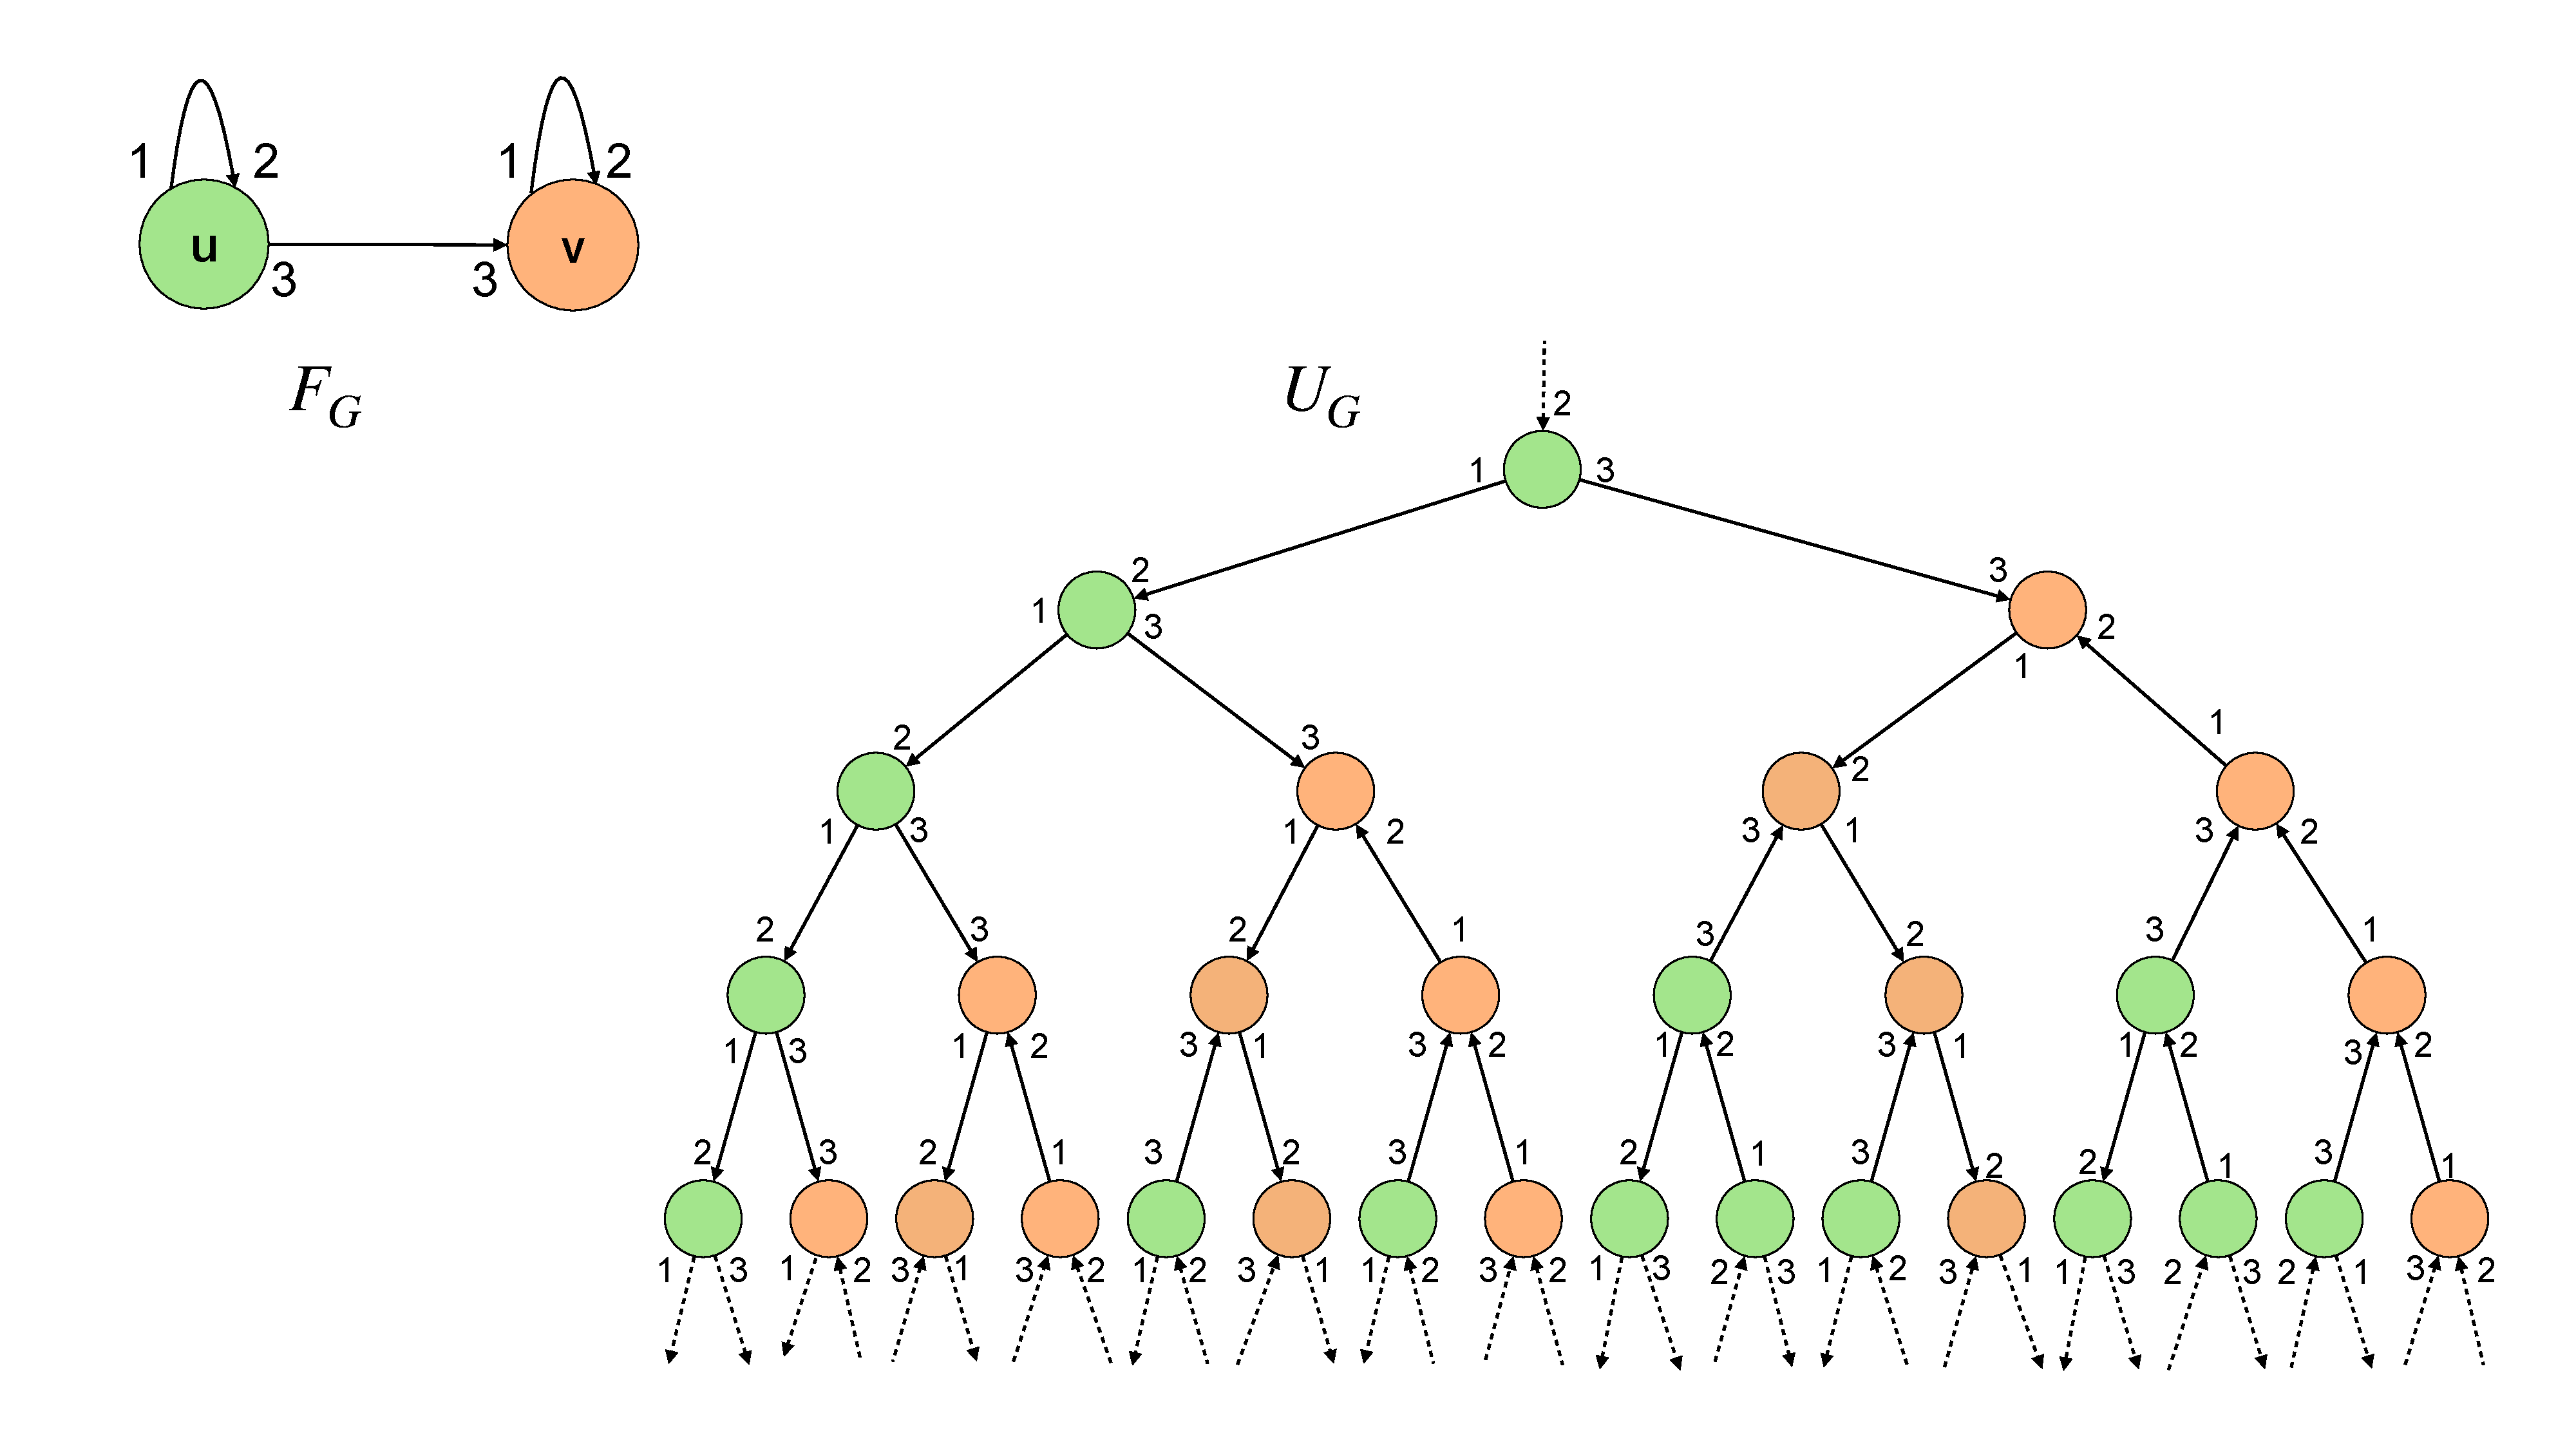
\includegraphics[scale = 0.22]{Figures/cover.pdf}
    \caption{$F_G$ and $U_G$}
    \label{fig:cv1}
\end{figure}

According to Jukka Suomela's textbook \cite{textbook}, we redefine here his definition of a covering map where the concerned graph's edges are oriented.
\begin{defi}
(Covering Map) Let $N = (V,P,p, \preceq)$ and $N' = (V',P',p',\preceq')$ be port-numbered networks whose edges are oriented, and let $\Phi: V \rightarrow V'$. We say that $\Phi$ is a covering map from $N$ to $N'$ if the following holds:
\begin{itemize}
    \item $\Phi$ is a surjection: $\Phi(V) = V'$
    \item $\Phi$ preserves degrees: $deg_N(v) = deg_{N'}(\Phi(v))$ for all $v \in V$.
    \item $\Phi$ preserves connections and port numbers: $p(u,i) = (v,j)$ implies
    $p'(\Phi(u), i) = (\Phi(v), j)$.
    \item $\Phi$ preserves orientations: $u \preceq v$ implies  $\Phi(u) \preceq' \Phi(v)$
\end{itemize}
\end{defi}
Theorem 8.1 of the textbook \cite[p.127]{textbook} also state that, if there exists a covering map $\Phi$ between two networks $N = (V,P,p, \preceq)$ and $N' = (V',P',p',\preceq')$, a deterministic algorithm that produce an output on $v \in V$ in $t=\mathcal{O}(1)$ must produce the same output for $v'\in V'$ after $t$ rounds if $v' = \Phi(v)$.\\\\
We now introduce $U_G = (V_U, E_U,\preceq_U)$ a tree that is the unfolded tree-like version of $F_G$ \cite[p. 7]{linear_in_delta} as in the figure \ref{fig:cv1}. We can see that a covering map between $F_G$ and $U_G$ exists.\\\\
 From this covering map, we know that :
 \begin{itemize}
     \item $A'$ must produce the same output for every node $u_i$ of $U_G$ that satisfy $u_i = \Phi(u)$
     \item $A'$ must produce the same output for every node $v_i$ of $U_G$ that satisfy $v_i = \Phi(v)$
 \end{itemize}
Hence, due to the port numbering of $F_G$, we can make the following requirements for $A'$ to produce a correct output:\\\\
$\exists u = (u_0,u_1,u_2),v = (v_0,v_1,v_2) \in W $ with $u_i,v_i\in \{A,B,C\}$ for $i\in \{0,1,2\}$ such that :
\begin{itemize}
    \item $\exists u_a,u_b \in u \hbox{ s.t. } (u_a,u_b)\in B$ with $a,b\in \{0,1,2\}, a\neq b$
    \item $\exists v_{a'},v_{b'} \in v \hbox{ s.t. } (v_{a'},v_{b'})\in B$ with $a',b'\in \{0,1,2\}, a'\neq b'$
    \item $(u_c,v_{c'})\in B$ where $c \in \{0,1,2\}$, $c\neq a, c\neq b$ and $c' \in \{0,1,2\}, c'\neq a', c'\neq b'$
\end{itemize}
In other words, for a node $u_i = \Phi(u)$ a configuration $u$ must exists such that $u_i$ can have 2 neighbors $u_a = \Phi(u)$ and $u_b = \Phi(u)$ and a neighbor $v_i = \Phi(v)$.
The sames goes for a node $v_i = \Phi(v)$ where a configuration $v$ must exists such that $v_i$ can have 2 neighbors $v_a = \Phi(v)$ and $v_b = \Phi(v)$ and a neighbor $u_i = \Phi(u)$.\\\\
If such requirements does not exists for a given problem, this implies that A' cannot have a correct output on $U_G$. By contraposition, $A$ must fails as well, we hence now that there exists a $\log^*(n)$ lower bounds on the complexity of the problem.
\begin{exmp}
Let's take the following problem that encode the maximal independent set : $\Pi=(3,2,W,B)$ with :
\begin{itemize}
    \item $W = AAA, BBB, BBC, BCC$
    \item $B = AB, CC$
\end{itemize}
For each white configuration, let's check if it match the requirements for $u$ or $v$:
\begin{itemize}
    \item \textbf{AAA} : AA is not in $B$, hence, a node labelled with AAA cannot have any neighbors labelled with the same configuration.
    \item \textbf{AAA} : BB is not in $B$, hence, a node labelled with BBB cannot have any neighbors labelled with the same configuration.
    \item \textbf{BBC} : there is neither BB neither BC in $B$, again, BBC cannot have any neighbors labelled with the same configuration.
    \item \textbf{BCC} : Here we can see that $CC\in B$, let hence put that $u = BCC$ and $v = BCC$ since its the only configuration that allows a nodes to have 2 neighbors with the same configurations. however, we can see that $BB$ is not in $B$, a node of type $u$ cannot have a neighbor of type $v$. BCC is not fulfilling the requirements.
\end{itemize}
No configuration fulfill the requirements, the problem has a $\log^*n$ lower bound.
\end{exmp}


\bibliographystyle{plain}
\bibliography{bib}
\end{document}